\documentclass{article}
\usepackage{amsmath, amsthm, amssymb, amsfonts}
\usepackage{thmtools}
\usepackage{graphicx}
\usepackage{setspace}
\usepackage{geometry}
\usepackage{float}
\usepackage{hyperref}
\usepackage[utf8]{inputenc}
\usepackage[english]{babel}
\usepackage{framed}
\usepackage[dvipsnames]{xcolor}
\usepackage{tcolorbox}
\usepackage{ dsfont }

\colorlet{LightGray}{White!90!Periwinkle}
\colorlet{LightOrange}{Orange!15}
\colorlet{LightGreen}{Green!15}

\graphicspath{ {./pictures/} }

\newcommand{\HRule}[1]{\rule{\linewidth}{#1}}

% ------------------------------------------------------------------------------

\begin{document}

% ------------------------------------------------------------------------------
% Cover Page and ToC
% ------------------------------------------------------------------------------

\title{ \normalsize \textsc{}
		\\ [2.0cm]
		\HRule{1.5pt} \\
		\LARGE \textbf{\uppercase{ AuD Hausübung von Blatt 5 }
        \HRule{2.0pt} \\ [0.6cm] \LARGE{ Hannes Albert } \vspace*{10\baselineskip}}
		}
\date{Mai 2023}
\author{\textbf{} \\
		Gruppe: 36 \\
		Tutor:  Julian Eulenburg}

\maketitle

\section{H1}
\setlength\leftskip{1cm}
\noindent a) \\
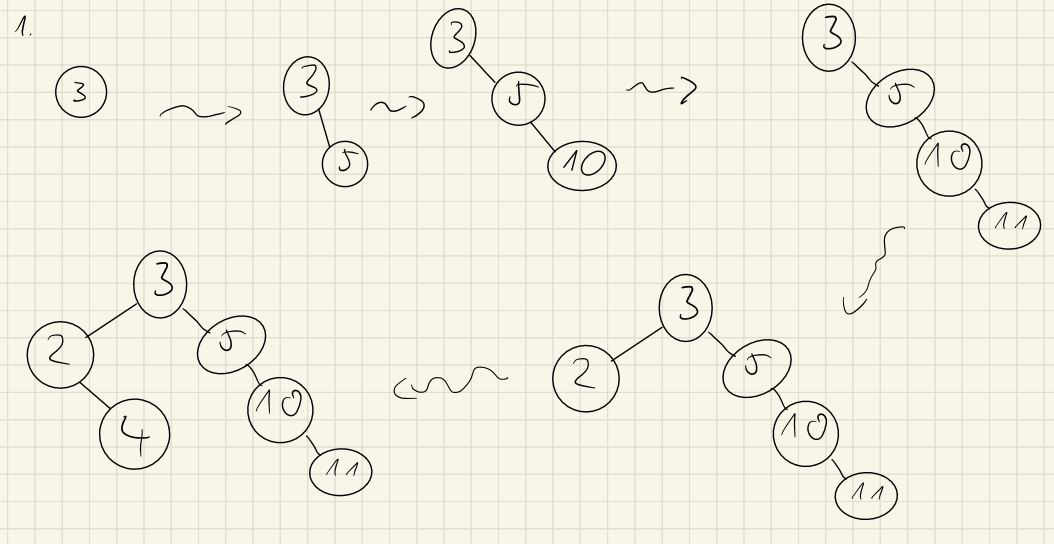
\includegraphics[scale=0.5]{ h1_a} \\ 
\bigskip
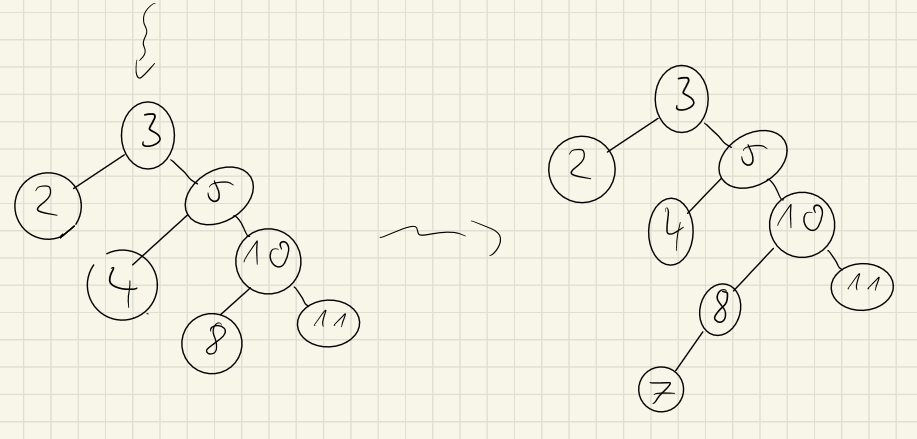
\includegraphics[scale=0.5]{ h1_a2} \\ 
\bigskip
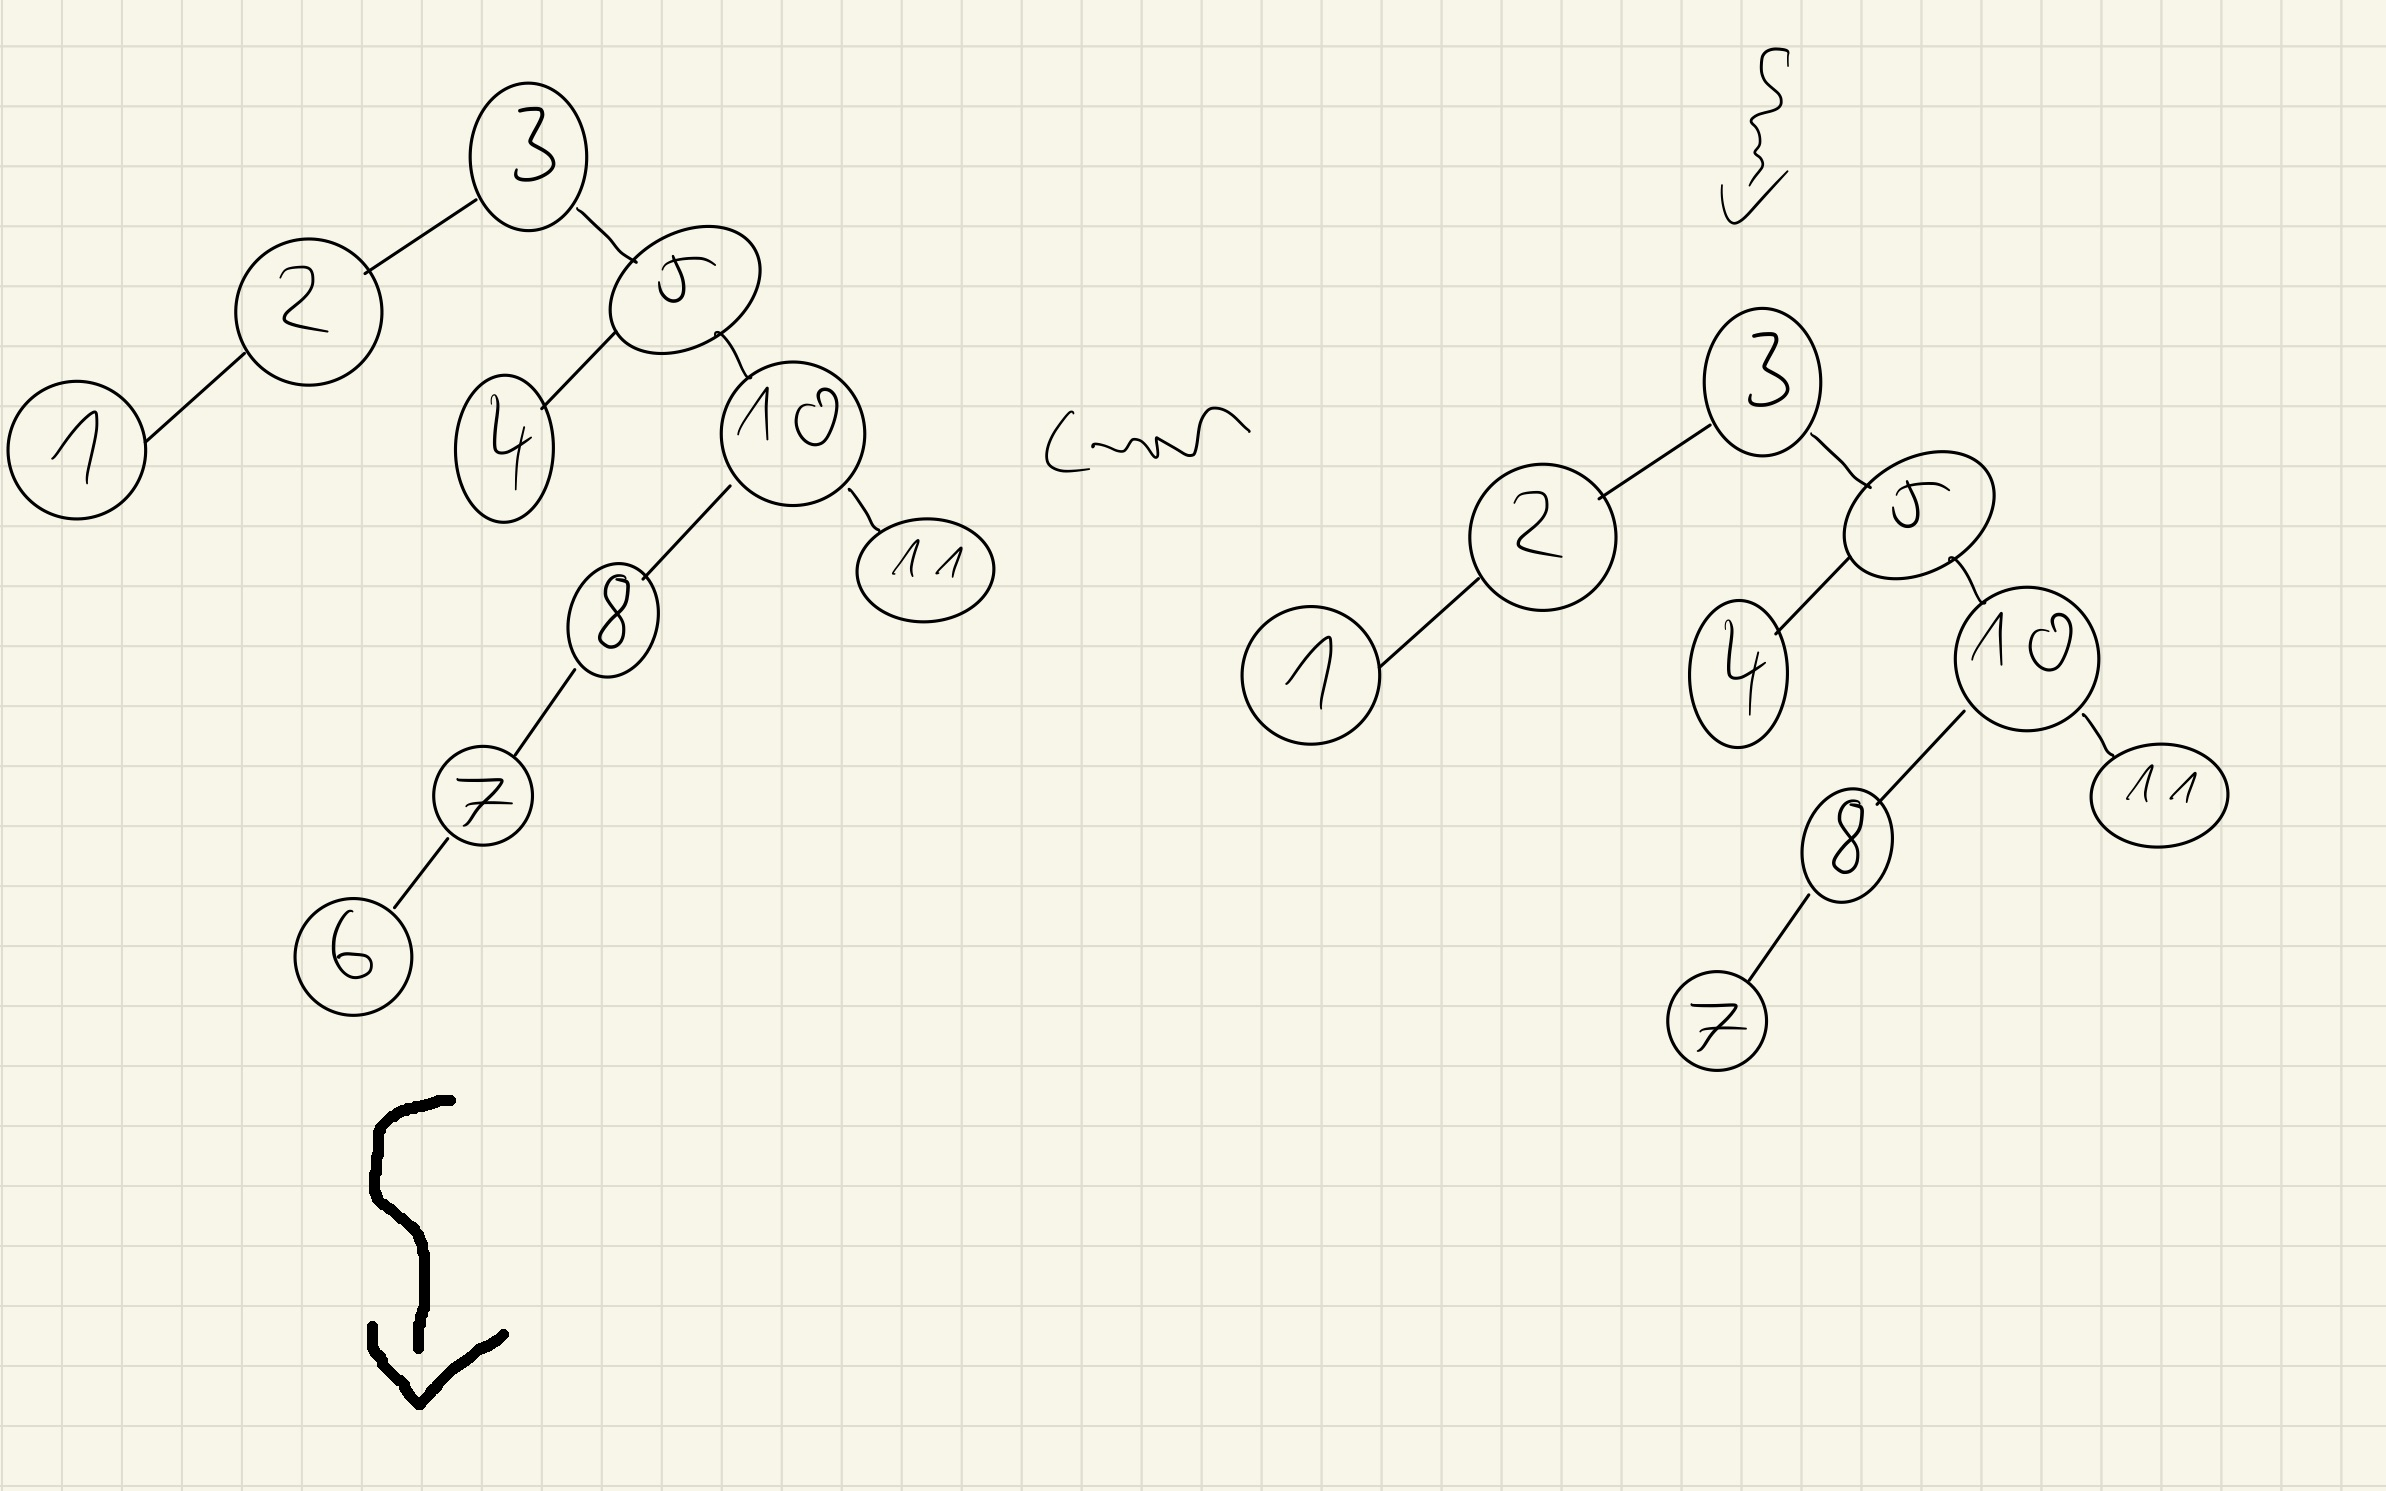
\includegraphics[scale=0.15]{ h1_a3 } \\ 
\bigskip
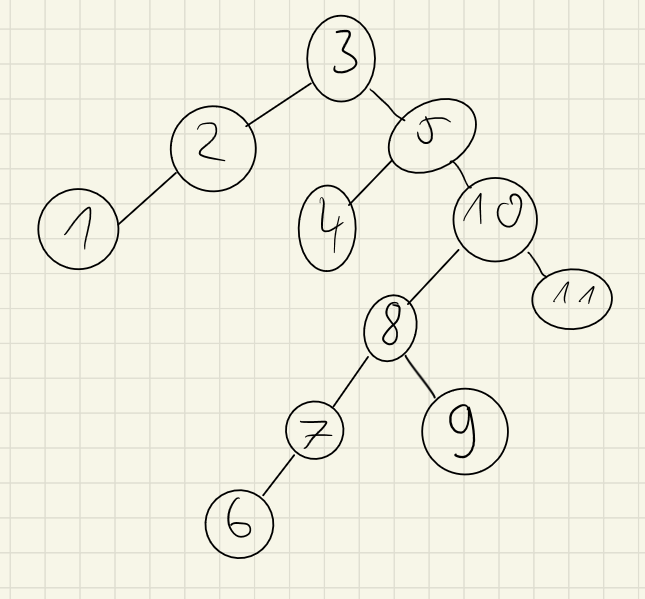
\includegraphics[scale=0.5]{ h1_a4 }  
\newpage 
\noindent b) \\
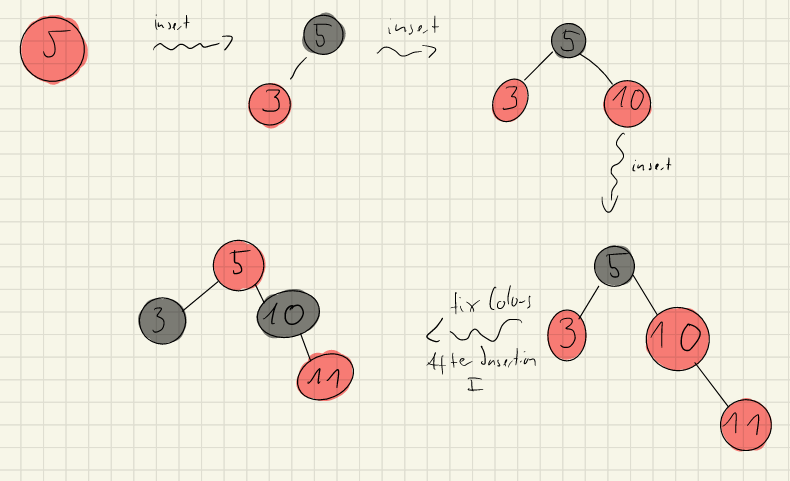
\includegraphics[scale=0.5]{ h1_a5 } \\
\bigskip
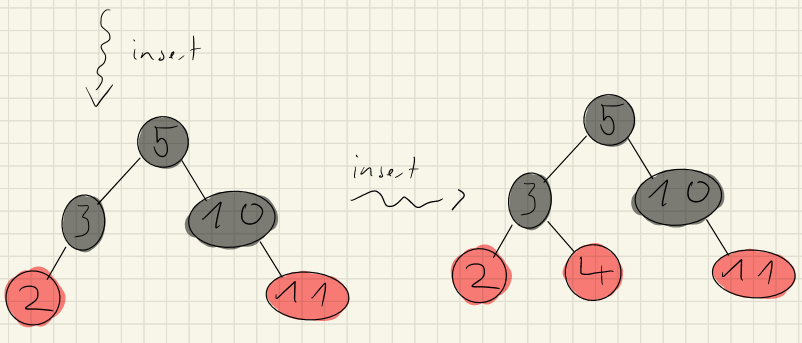
\includegraphics[scale=0.5]{ h1_a6 } \\
\bigskip
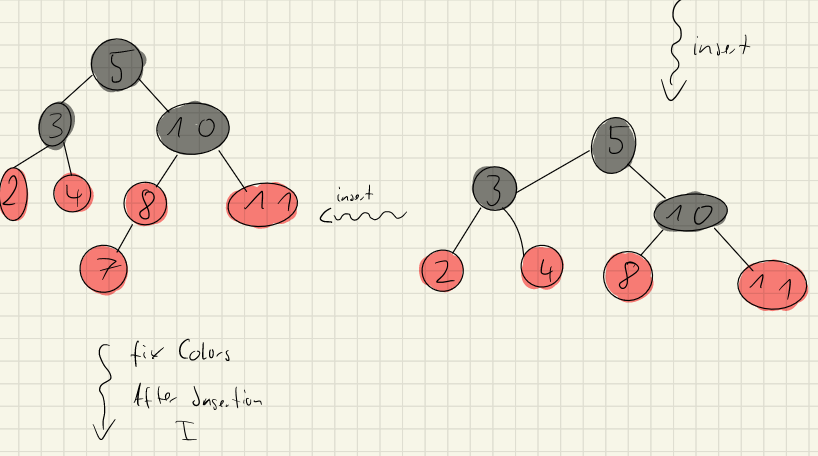
\includegraphics[scale=0.5]{ h1_a7 } \\
\bigskip
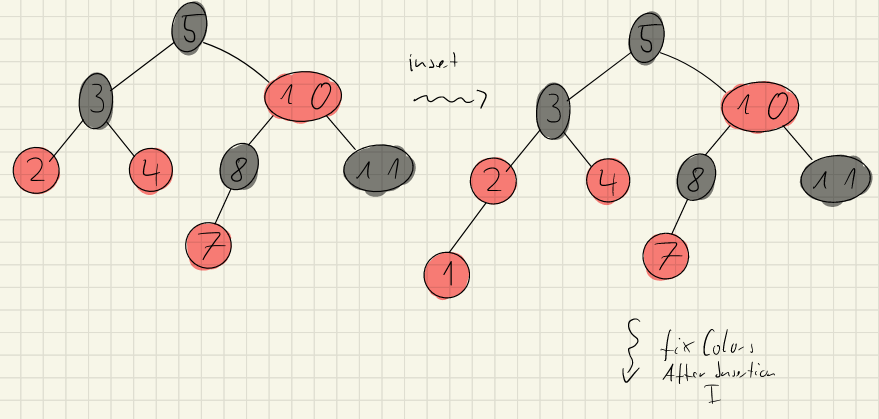
\includegraphics[scale=0.5]{ h1_a8 } \\
\bigskip
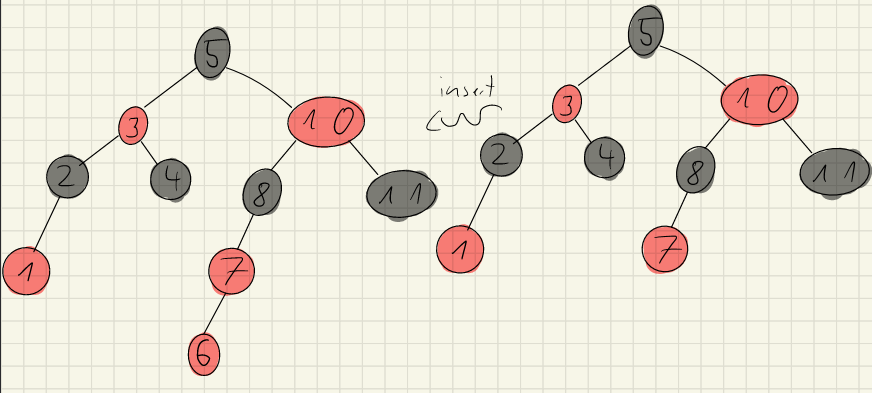
\includegraphics[scale=0.5]{ h1_a9 } \\
\bigskip
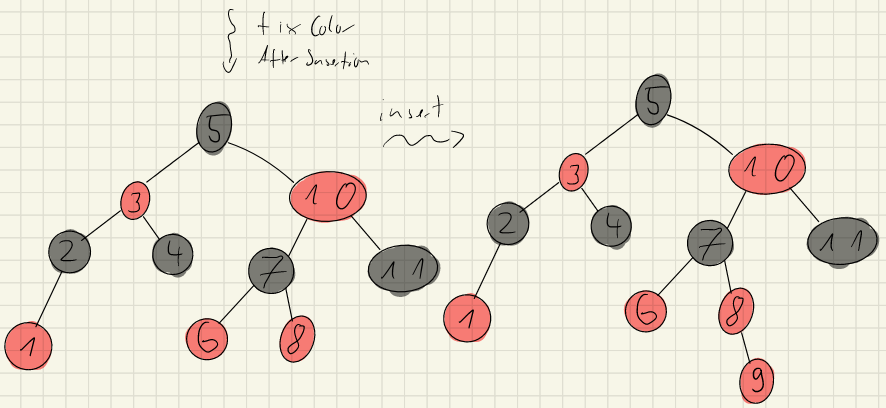
\includegraphics[scale=0.5]{ h1_a10 } \\
\bigskip
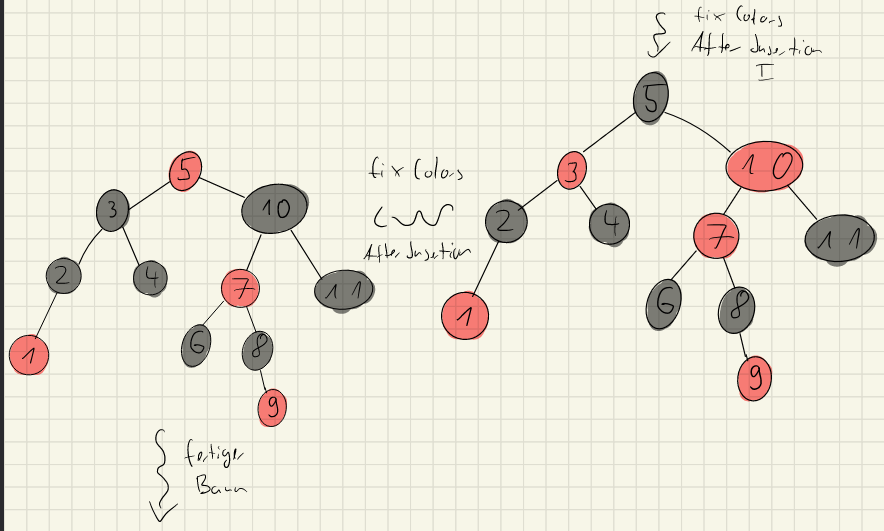
\includegraphics[scale=0.5]{ h1_a11 } \\
\bigskip
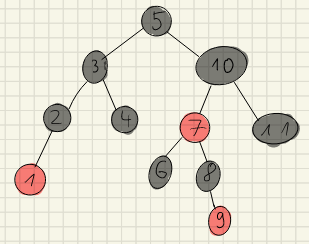
\includegraphics[scale=1]{ h1_a12 } \\
\bigskip
Mithilfe der Algorithmen von Foliensatz 03, S. 47 + 51 erhalten wir für den BST aus Aufgabe H1 a) folgenden Reihenfolgen 
für die verschiedenen Traversierungs-Möglichkeiten:
\begin{align*}
    Preorder: \text{ 3 2 1 5 4 10 8 7 6 9 11} \\ 
    Inorder: \text{1 2 3 4 5 6 7 8 9 10 11} \\ 
    Postorder: \text{1 2 4 6 7 9 8 11 10 5 3} \\ 
\end{align*}
\newpage
Für den Rot-Schwarz-Baum hingegen erhalten wir die folgenden Reihenfolgen:
\begin{align*}
    Preorder: \text{5 3 2 1 4 10 7 6 8 9 11} \\
    Inorder: \text{1 2 3 4 5 6 7 8 9 10 11} \\ 
    Postorder: \text{1 2 4 3 6 9 8 7 11 10 5} \\ 
\end{align*}

\noindent d) 
Wir Löschen die Blätter nacheinander wie folgt: \\ 
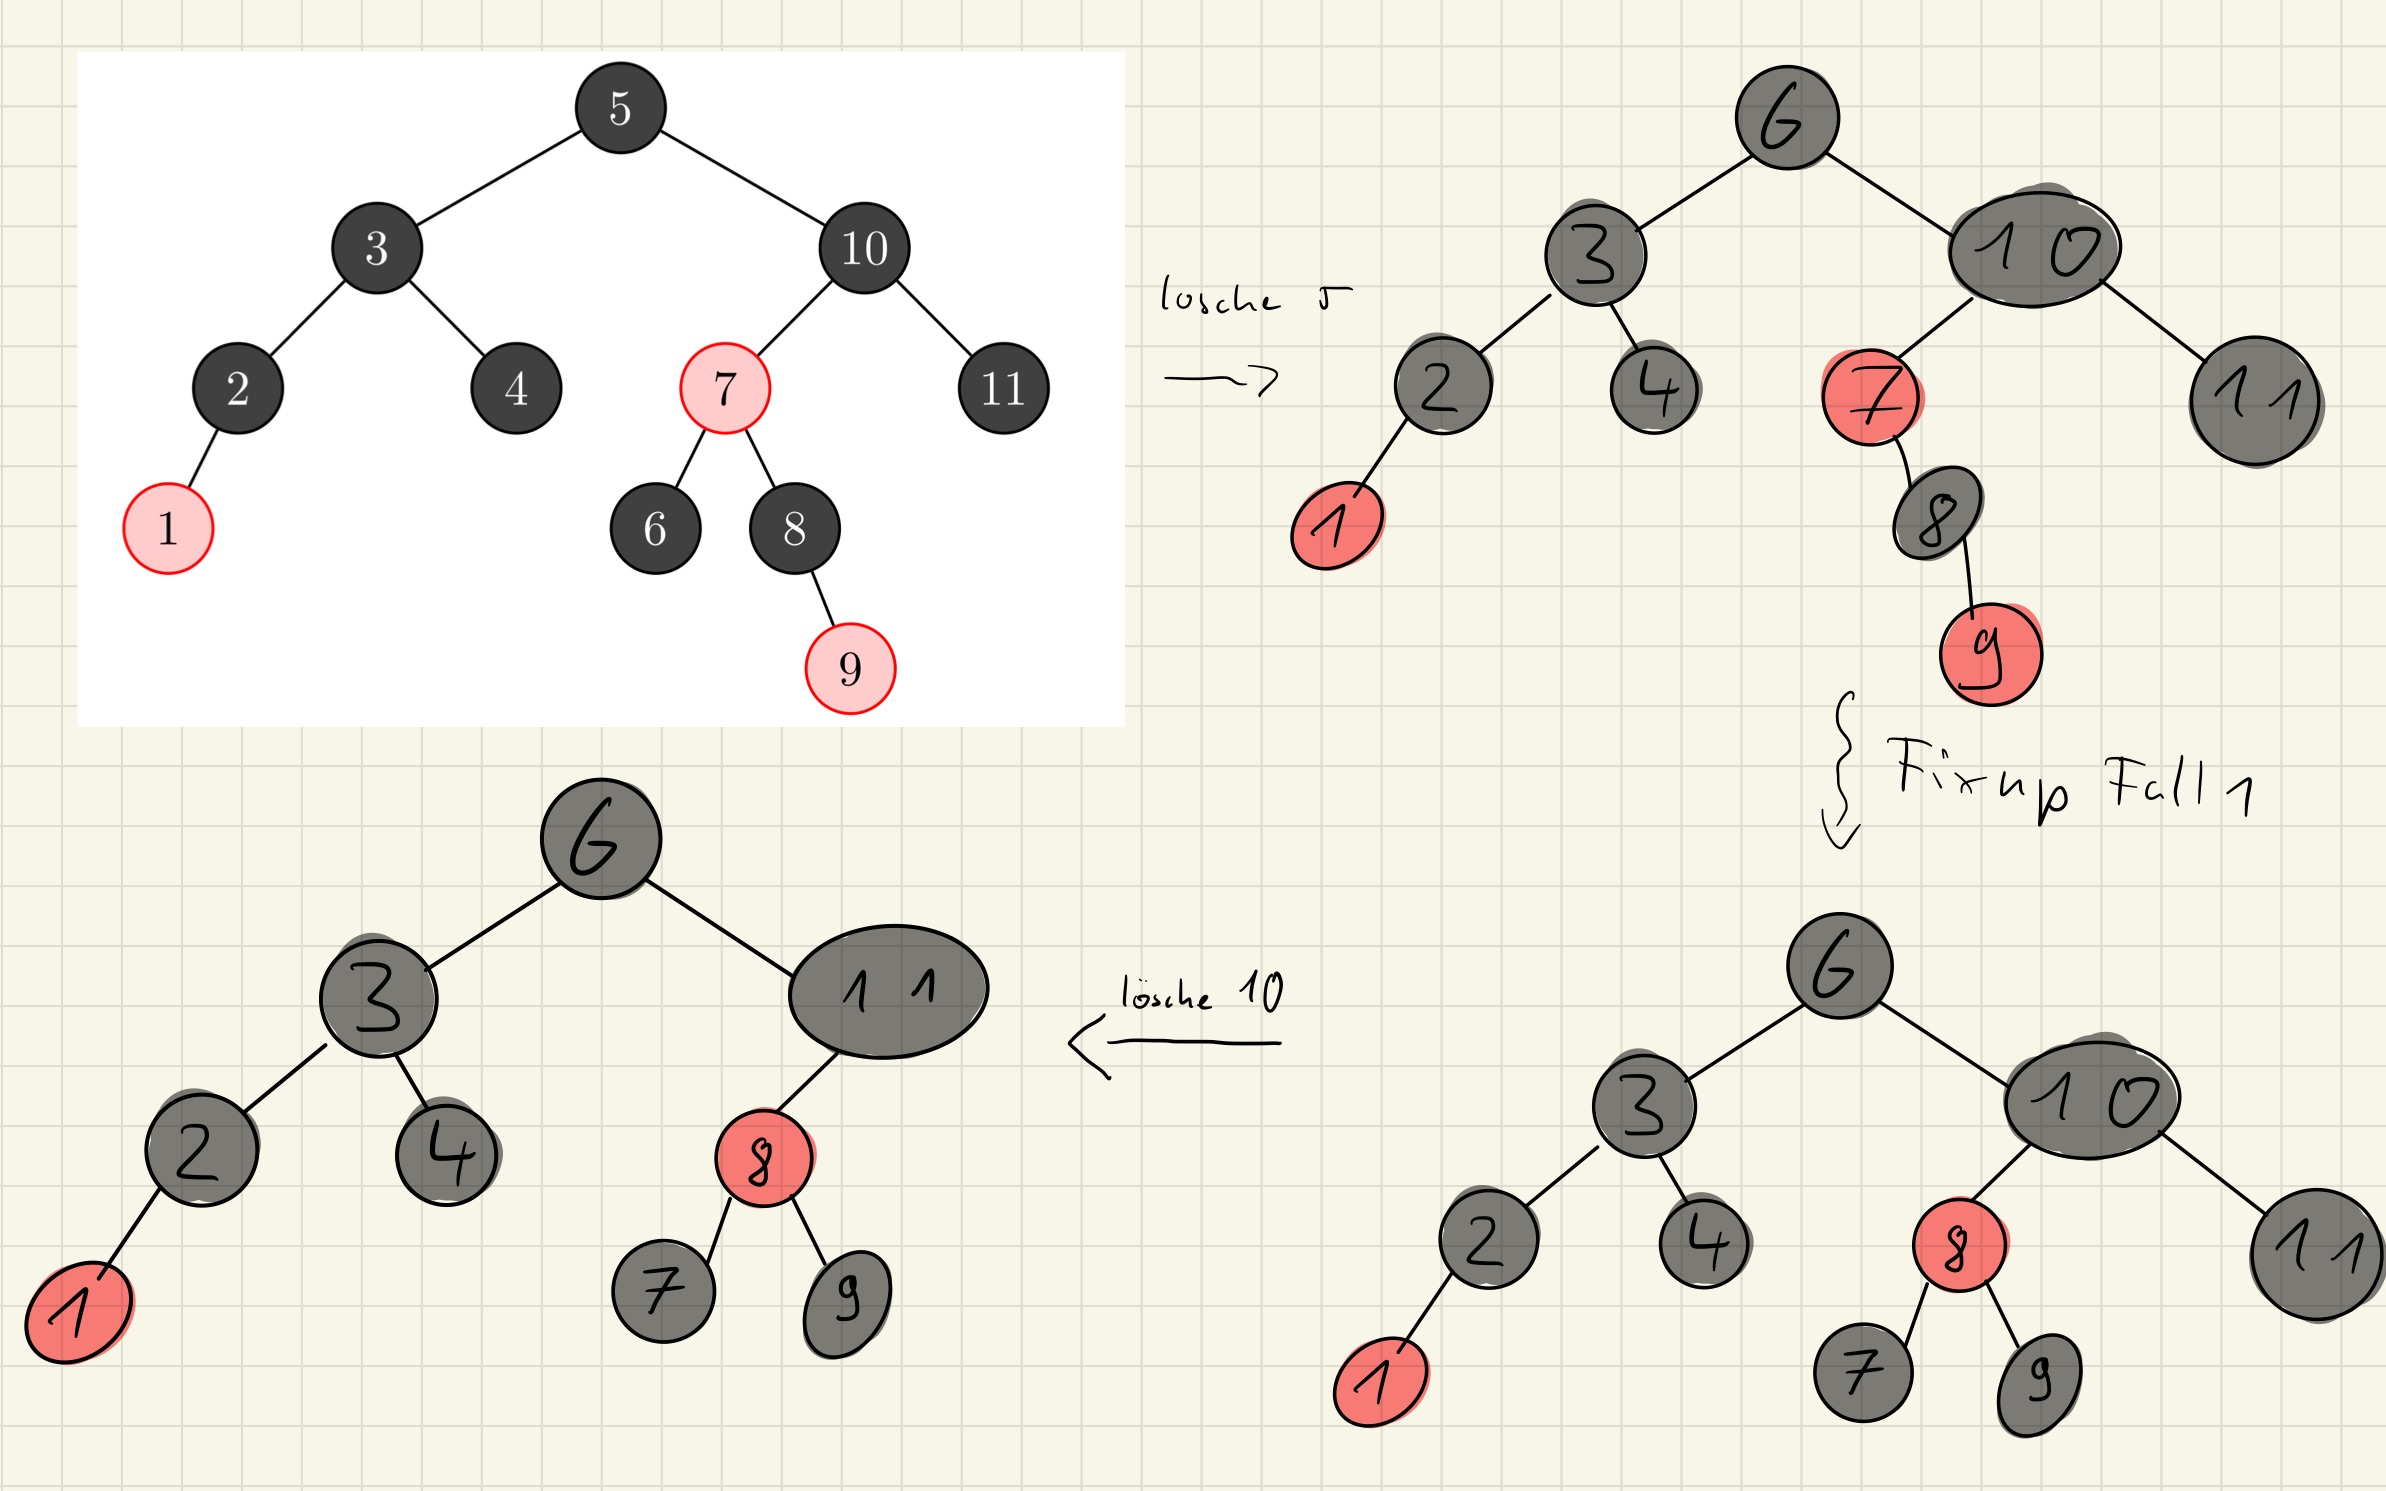
\includegraphics[scale=0.15]{ h1_a13 } \\ 
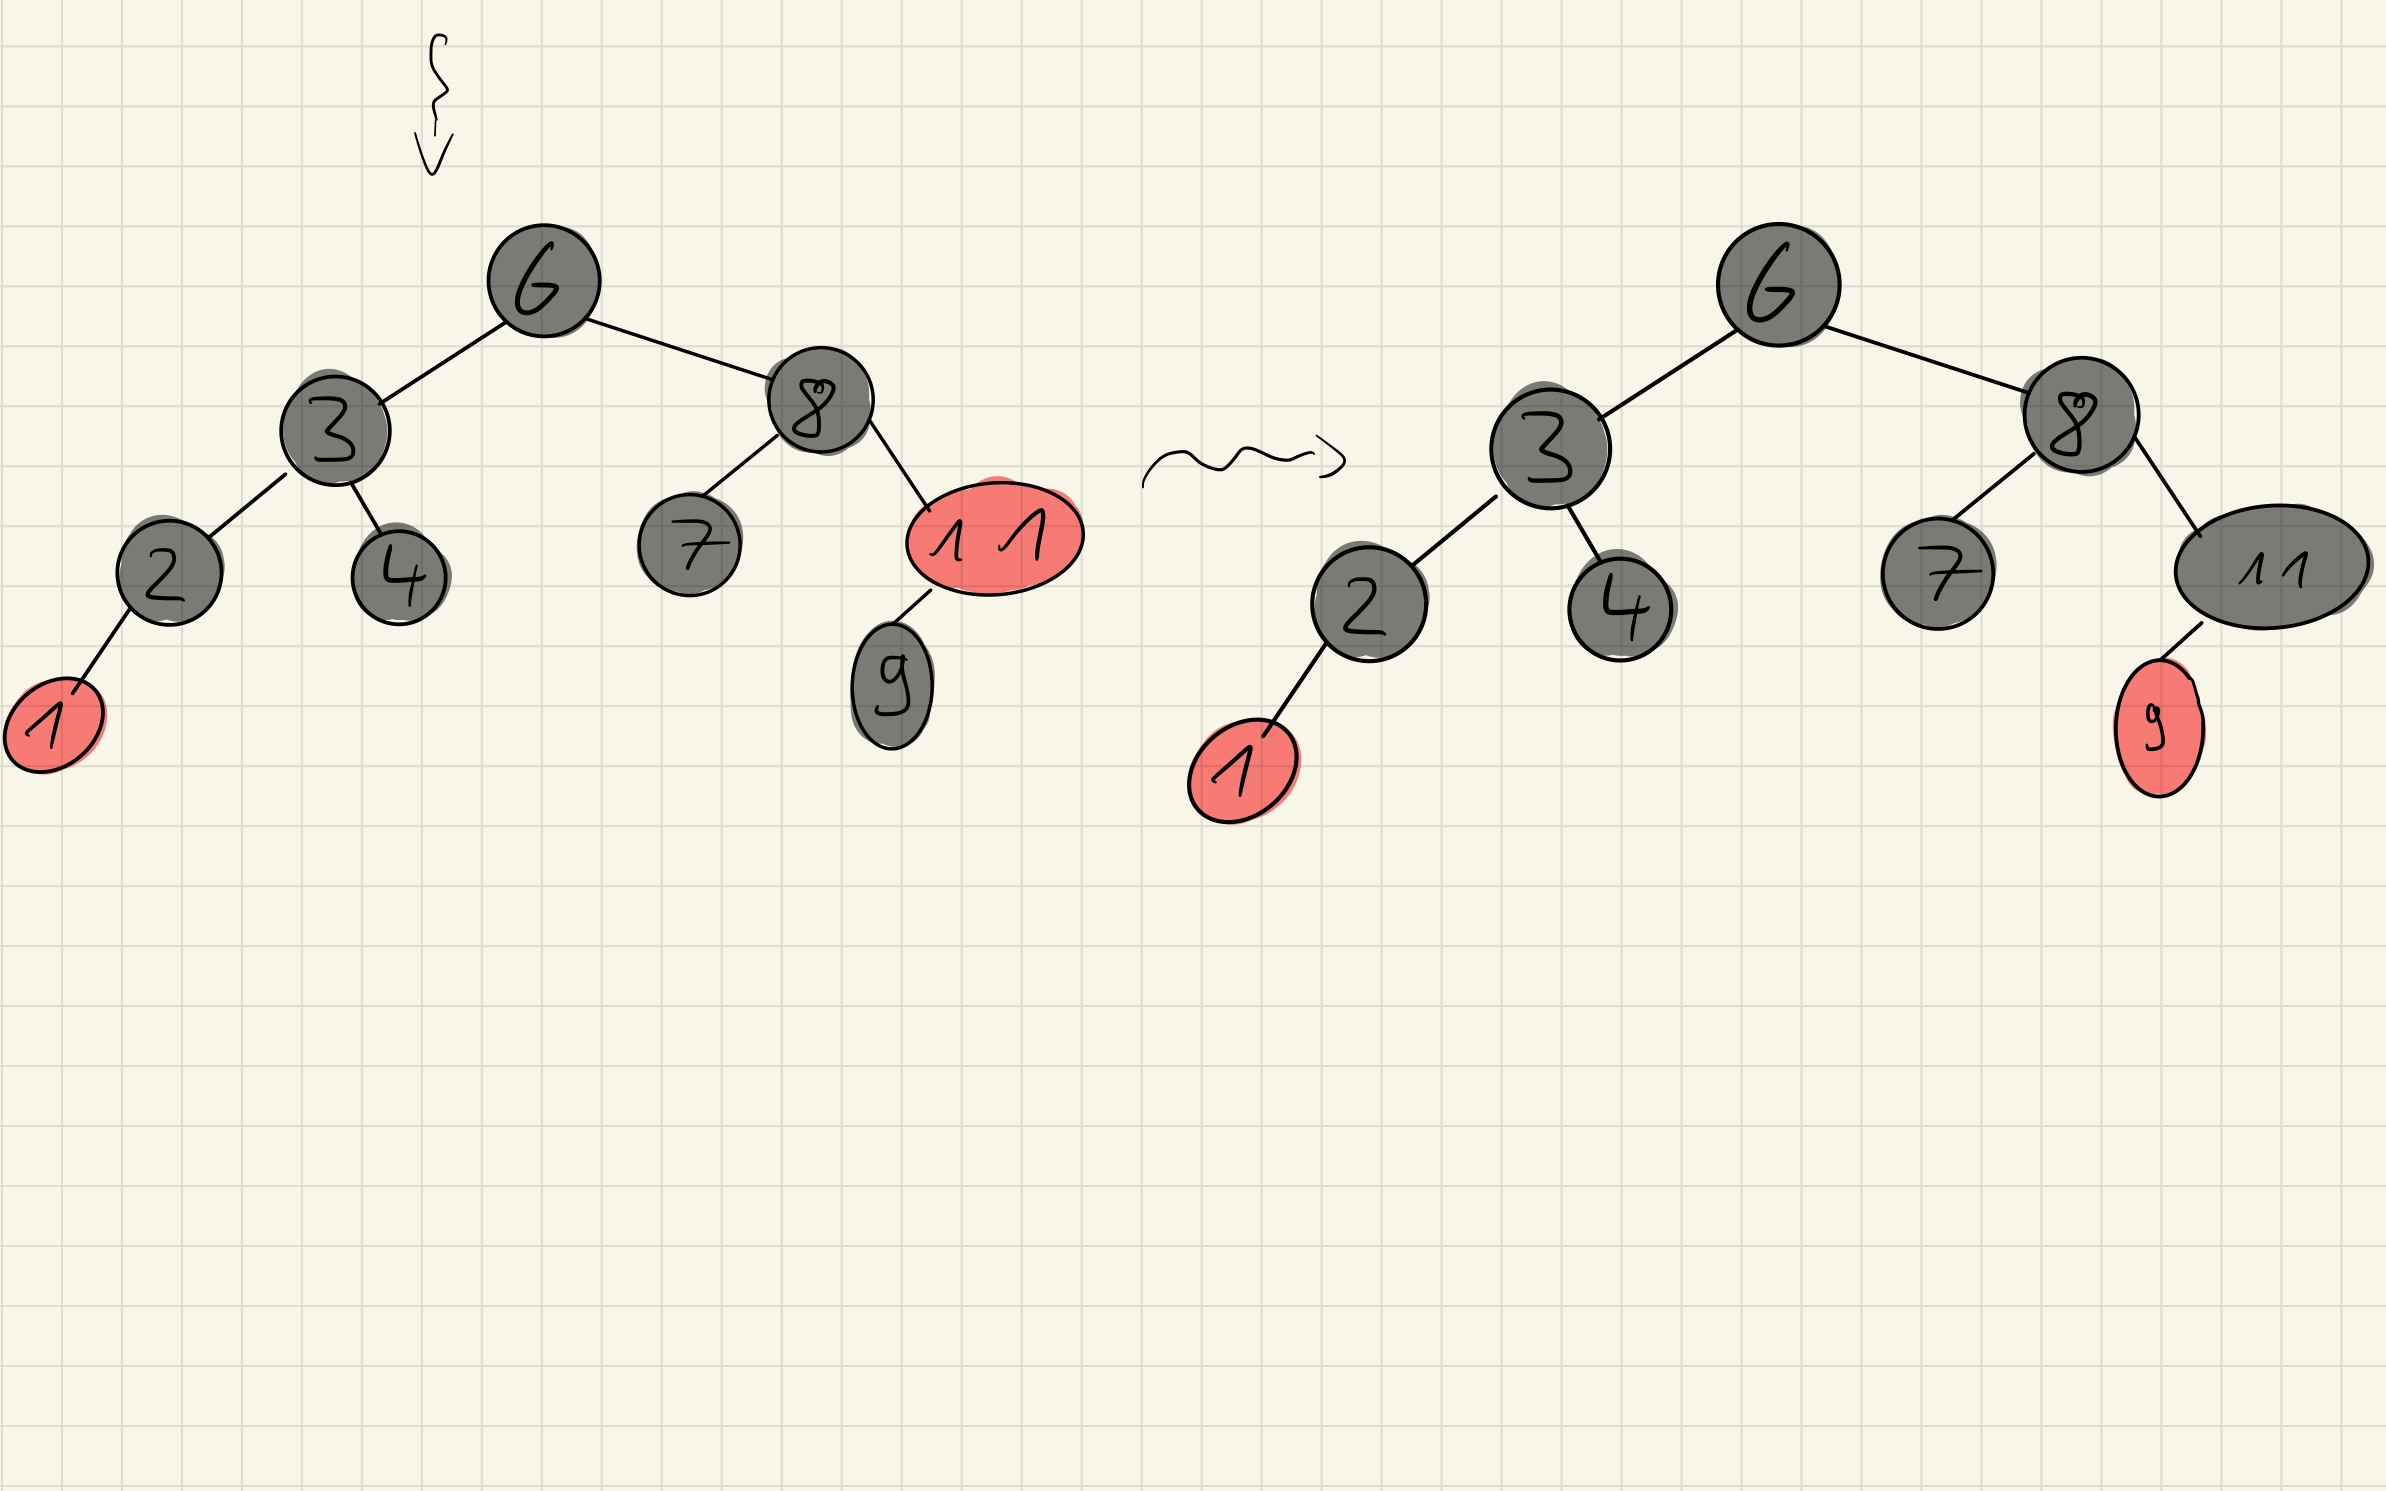
\includegraphics[scale=0.15]{ h1_a14 } \\  
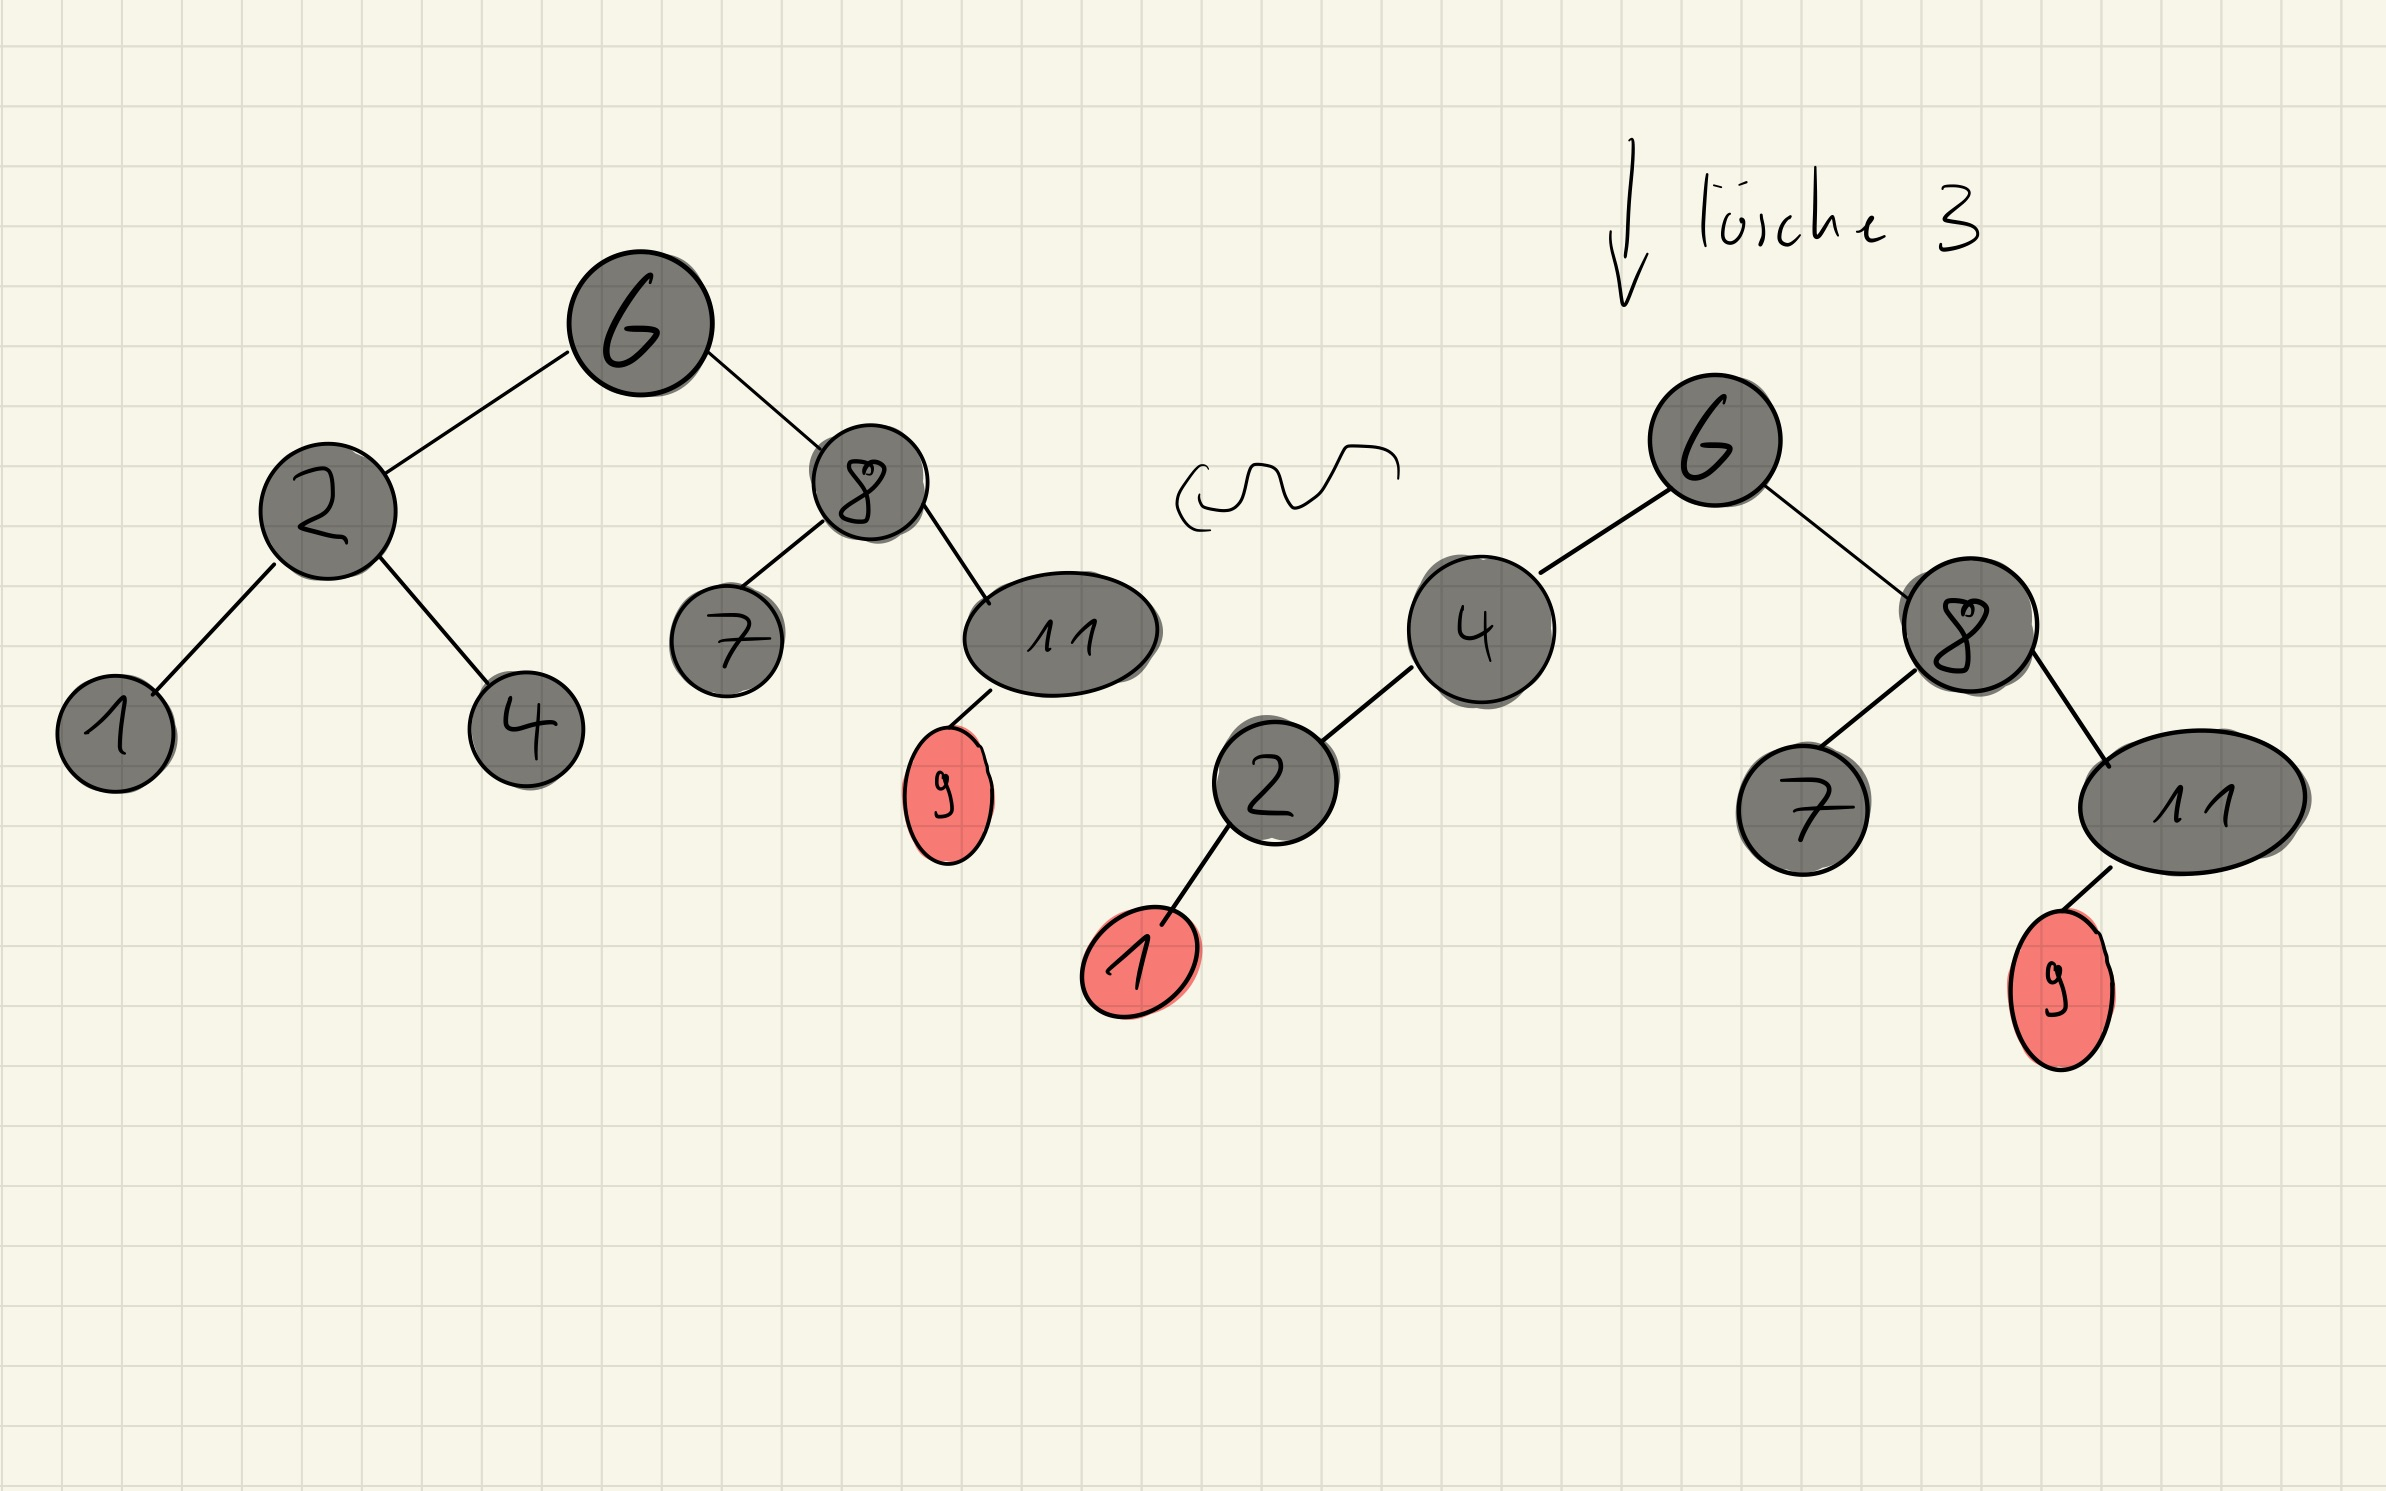
\includegraphics[scale=0.15]{ h1_a14a } 

\section{H2}
\noindent a) \\ 
Induktionsanfang: \\ 
\indent Sei n = 1. Da ein einzelner Knoten keine Kanten hat, da es ja schließlich keine Knoten 
\indent zum verbinden gibt. D.h. Anzahl der Knoten entspicht 0.
gilt die Formel: 
\[
    n - 1 \overset{n = 1}{=} 1 - 1 = 0
\]
Induktionsvorraussetung: \\
\indent Sei n $\in$ $\mathds{N}^*$, die Anzahl der Knoten eines Baumes. So entspricht die Anzahl der Kanten
in einem Baum n - 1. \\ 
Induktionsschritt: \\ 
Für den Induktionsschritt setzen wir die Anzahl der Knoten auf n + 1 für n $\in$ $\mathds{N}^*$
\[
    n + 1 \overset{IV}{=} n - 1 + 1 = n
\]
Die Fomel wurde hiermit gezeight, da (n + 1) - 1 = n und wir sind fertig. \indent $\square$ 

\bigskip
\noindent b) \\ 
Die Best-Case Laufzeit erhalten wir unter der Annahme, dass durch das Einfügen aller
Knoten ein möglichst ausgeglichener Baum entsteht. Damit erhalten wir für die Laufzeit der 
Einfügeoperation n * O($log_2$ n) = O(n $log_2$ n) (Foliensatz 03, S. 81) und für die Inorder-Traversierung erhalten wir 
eine Laufzeit von O(n) (Foliensatz 03, S. 48). Damit gilt:
\[
    O(n*log_2 n) + O(n) = O(n*log_2 n + n) = O(n * log_2 n)
\]
Somit erhalten wir eine Best-Case Laufzeit von O(n $log_2$ n).
Im Falle der Worst-Case Laufzeit entsteht durch die Einfüge-Operationen im degenerierten Sinne 
eine lineare Liste was insgesamt zu einer Laufzeit von n * O(n) = O($n^2$) führt. Für die Inorder-Traversierung 
erhalten wir weiterhin O(n). Damit bekommen wir:
\[
    O(n^2) + O(n) = O(n^2 + n) = O(n^2) 
\]
Also ergibt sich für die Worst-Case Laufzeit O($n^2)$.
\bigskip
\noindent c) \\ 
Wir verwenden die gleiche Namensgebung für die beteiligten Elemente 
wie die Folien: \\
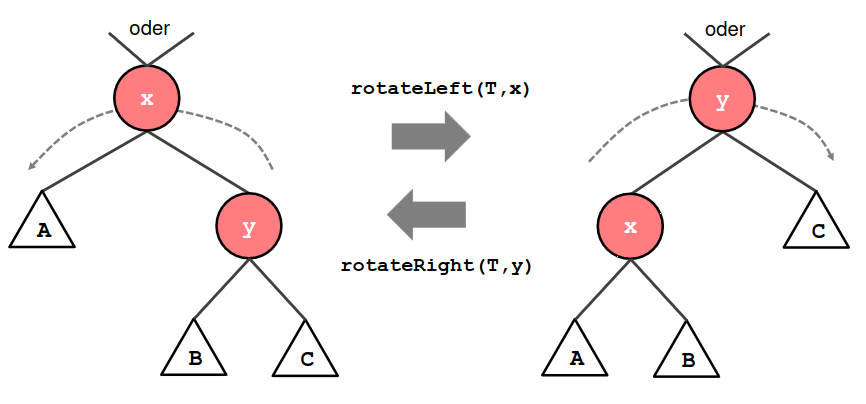
\includegraphics[scale=0.5]{ h1_a15 } \\ 
\bigskip
Um zu zeigen, dass die BST-Eigenschaften erhalten bleiben müssen wir zeigen,
dass nach der Rotation folgende Eigenschaften gelten:
\begin{enumerate}
    \item $\forall k \in A : k.key <= x.key$  
    \item $\forall k \in B \cup C \cup \{y\} : k.key >= x.key$
    \item $\forall k \in B : k.key <= y.key$
    \item $\forall k \in C : k.key >= y.key$
    \item x.key $<=$ x.parent.key $\vee$ x.key $>=$ x.parent.key \text{,  falls T.root != x} 
\end{enumerate}

\smallskip
\noindent Nun arbeiten wir die einzelnen Punkte der Reihe nach ab: \\  
1. \\ 
\setlength\leftskip{1.5cm}
Da bereits vor der Rotation A der linke Teilbaum von x war 
müssen die geforderten Eigenschaften schon vor der Rotation gültig 
gewesen sein und da sich für den Teilbaum nichts geändert hat sind
sie es weiterhin. \\ 

\smallskip
\noindent 2. \\ 
Da B vor der Rotation der rechte Teilbaum von x war, gilt auch nach der 
Rotation, dass der Schllüssel aller Knoten in B größer gleich dem Wert 
des Knoten von x ist.
Da x vor der Rotation Teil des linken Teilbaums von y war gilt: x.key $<=$ y.key.
Das heißt, dass y.key $>=$ x.key, weshalb die von uns geforderte Eigenschaft
erfüllt ist.
Da C vor der Rotation Teil des rechten Teilbaums von y war gilt nach 
der Rotation:
\[
    \forall k \in C : y.key <= k.key
\]
Das bedeutet auch x.key $<=$ y.key $<=$ k.key für alle k $\in$ C.
Somit ist auch die zweite Eigenschaft nach der Rotation erfüllt. \\ 

\smallskip
\noindent 3. \\ 
Da B vor der Rotation auch schon Teil des linken Teilbaums von y war, 
gilt bereits für alle Elemente von B, dass ihr Schlüsselwert kleiner ist 
als der von y. Dies ist logischerweise auch nach der Rotation schon so. \\ 

\smallskip
\noindent 4. \\ 
Da C vor der Rotation der rechte Teilbaum von y war und dies sich während 
der Rotation auch nicht geändert hat gilt dies natürlcih auch noch 
nach Rotation, weshalb dieser Punkt auch erfüllt ist.

\smallskip 
\noindent 5. \\ 
Wir treffen hier eine Fallunterscheidung: \\ 
1.Fall: x.parent.left = x \\ 
Da x vor der Rotation Teil des linken Teilbaums war, gilt auch weiterhin,
dass x.key <= x.parent.key. \\ 
2.Fall: x.parent.right = x \\
Da x vor der Rotation Teil des rechten Teilbaums war, gilt auch weiterhin,
dass x.key >= x.parent.key. \\ 
Somit ist auch die fünfte geforderte Eigenschaft erfüllt und wir sind fertig.

\bigskip
\noindent Damit eine Rechtsrotation funktioniert muss natürlich gelten, dass x und y ungelich nil sind.
Bei A, B und C ist dies nicht so wichtig: wenn der Teilbaum nicht existiert gibt 
es keine Elemente deren Schlüssel größer, kleiner oder gleich x.key oder y.key sein können.
Dementsprechend würde für A = nil 1. außer Acht gewerden lassen können.
Für B = nil könnte 3. ignoriert werden und in 2. würde einfach B durch die Menge ohne Elemente 
ersetzt werden. Gleiches gilt für den Fall, dass C = nil wäre, wobei dann 4. ignoriert werden könnte.
\end{document}

